
\documentclass{article}

% if you need to pass options to natbib, use, e.g.:
% \PassOptionsToPackage{numbers, compress}{natbib}
% before loading nips_2017
%
% to avoid loading the natbib package, add option nonatbib:
% \usepackage[nonatbib]{nips_2017}

\usepackage{nips_2017}

% to compile a camera-ready version, add the [final] option, e.g.:
% \usepackage[final]{nips_2017}

\usepackage[utf8]{inputenc} % allow utf-8 input
\usepackage[T1]{fontenc}    % use 8-bit T1 fonts
\usepackage{hyperref}       % hyperlinks
\usepackage{url}            % simple URL typesetting
\usepackage{booktabs}       % professional-quality tables
\usepackage{amsfonts}       % blackboard math symbols
\usepackage{nicefrac}       % compact symbols for 1/2, etc.
\usepackage{microtype}      % microtypography

\usepackage{graphicx}

\title{Anime Artist Analysis based on CNN}

% The \author macro works with any number of authors. There are two
% commands used to separate the names and addresses of multiple
% authors: \And and \AND.
%
% Using \And between authors leaves it to LaTeX to determine where to
% break the lines. Using \AND forces a line break at that point. So,
% if LaTeX puts 3 of 4 authors names on the first line, and the last
% on the second line, try using \AND instead of \And before the third
% author name.

\author{Ziyi Chen \\
  Computer Science  \\
  UC Santa Cruz\\
  {\tt zchen139@ucsc.edu} \\\And
   Chujiao Hou\\
  Computer Science  \\
  UC Santa Cruz\\
  {\tt chou8@ucsc.edu} \\\And
   Xinyuan Ma\\
  Computer Engineering  \\
  UC Santa Cruz\\
  {\tt xma34@ucsc.edu} \\}
  
  

\begin{document}
% \nipsfinalcopy is no longer used

\maketitle

\begin{abstract}
Artist recognition is not easy for human beings if the artworks are general and share many similarities, but modern machine learning or deep learning models may help people identify the artwork authors. In this project, we trained Convolutional Neural Networks (CNN) identifying Japanese anime artists. Our dataset was crawled from Pixiv, a well-known Japanese website containing lots of fine anime artworks. Specifically, the dataset has 9 authors and each one has 200 paintings. We trained different kinds of networks, from a very basic Conv2D net to more advanced networks, in order to carry out the identification. It turned out that traditional neural networks can in some way identify different authors, but the accuracy could be improved to a better level by tuning hyperparameters or using more advanced networks such as ResNet and VGGNet.

\end{abstract}

\section{Introduction}
Pixiv is a Japanese online community for artists, launched on September 10, 2007, by Takahiro Kamitani. Pixiv aims to provide a place for artists to exhibit their illustrations and get feedback via a rating system and user comments. As of September 2016, the site consists of over 43 million illustration submissions.

Artist identification has very different difficulties. Some classic artworks by very famous artists like Van Gogh, Monet, or Pablo Picasso, have very distinguished artists’ personal styles and painting structures. These artworks’ authors may be easier for both human beings and neural networks to identify. But the problem lies in many modern arts like Japanese animes. There are great works and unique styles but many more artworks are highly similar. Even well-known comics artists draw people, scenery or still lives alike. To make things worse, many artists no longer draw in traditional ways such as pen and brush. Many artists especially young ones like sharing paintings across the internet. In order to conveniently spreading their work, they are more likely to directly draw pictures on the computer with equipment like digital panels or handwriting pads.

We want to concentrate on illustrations of Japanese anime, which have a similar style as a whole. But there are still differences between every artist, like color preference, brushwork and painting structures. Previous work on artist recognition was done by specialists in artworks, or computer scientists who had a good comprehension of art, and they typically selected feature representations manually and used these features to build supervised learning models. But in our project, based on the hypothesis that every artist has unique styles and characteristics, even if differences are very latent, we trained CNNs for this problem. It is likely that CNNs can identify best representations of features as they are trained.

Also, it is highly possible that simple Con2D net could not perform well and reach the required accuracy, we also consider building other CNN models like VGGNet and ResNet, which could build deeper and more efficient networks. By starting with basic Con2D net and only two author identification, we do this project step by step to make the model more complicated and add more authors to be identified.


\section{Related work}

Previously many work on artists identification was done by humans. The first several attempts to make machine do this task were based on manually selected features such as brush strokes, although this kind of learning algorithms aims at style identification rather than artists identification. Many image features have been used, including scale-invariant feature transforms (SIFT), histograms of oriented gradients (HOG), and more [3, 16, 19, 20]. Prior work typically used supervised learning algorithms such as SVMs to identify artist and style given these features. Other classification methods such as k-nearest neighbors and hierarchical clustering have been used as well.

Maximum Likelihood Image Identification and Restoration Based on the expectation maximum (EM) Algorithm, proposed by A.K. Katsaggelos, showed that expectation maximum algorithm is a powerful iterative procedure for computing machine learning estimates of unknown parameters involved in the likelihood function of the observed data[1]. Deep Residual Learning for Image Recognition[2], presented a residual learning framework to ease the training of networks that are substantially deeper than those used previously; this paper explicitly reformulated the layers as learning residual functions with reference to the layer inputs, instead of learning unreferenced functions, which provide a new idea for us.

And for image clustering, Spatial Models for Fuzzy Clustering proposed by Dzung L. Pham, proposing a novel approach to fuzzy clustering for image segmentation where a new objective function is proposed for incorporating spatial context into fuzzy C-means algorithm[3]. Image Clustering using Local Discriminant Models and Global Integration, by Yi Yang , Dong Xu, Feiping Nie, Shuicheng Yan, YueTing Zhuang, they constructing a local clique comprising the data point and its neighboring data points, and using a local discriminant model for each local clique to evaluate the clustering performance of samples within the local clique[4]. 

Recently, CNN has been proved to be quite efficient and accurate on many image recognition tasks. After trained under properly selected parameters, CNNs can successfully decompose artworks especially paintings into style and content components. They can even transfer style from one painting to another and there are already many fancy applications such as Prisma. This implies that CNNs can capture artwork styles.

\section{Dataset}
\subsection{Crawling}
The image dataset is crawled from Pixiv (\url{https://www.pixiv.net/}). We first use a chrome extension called Pxer, which can be used under the webpage of a certain artist and crawls all image URL of the artist. We randomly select 16 artists who have uploaded more than 200 illustrations and use Pxer to get URL. We tried to use downloader like Thunder to batch download pictures, but it failed. Because Pixiv forbids to access the image directly using the URL without referring to the HTTP head. Then we used Python and imitated the HTTP head to crawl illustrations. We have more than 5000 origin images from 16 different authors. Samples of illustrations are shown in Figure \ref{pixiv_sample}.

\begin{figure}[ht]
  \centering
  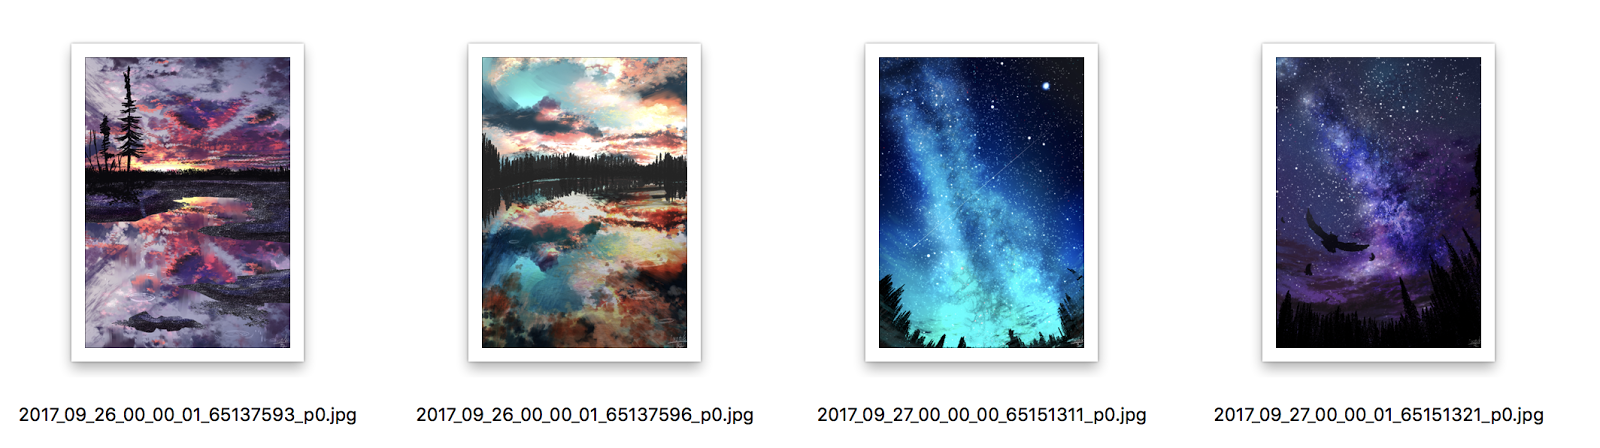
\includegraphics[width=0.94\linewidth]{pixiv_sample.png}
  \caption{Samples of illustrations from Pixiv.}
  \label{pixiv_sample}
\end{figure}

\subsection{Image Proprecessing}
Compressing and cropping images is an important step in image preprocessing. 
The size of images varies from 50 kilobytes to 3 megabytes.  We first deleted the pictures without characteristics of the painter (such as blank pages, advertisements, etc.). We used two different ways to process the image.

The first is to rescale image. Through OpenCV, we compressed the picture to the size of $500 \times 500$ pixels. After that, we manually selected the picture which is obviously distorted after being compressed and then deleted them. But it may lose the pixel information of images.

The second wat is to crop the image from center as shown in \ref{crop_sample}. Since some image is quite large and the important information of the image is more likely to be in the center of the image. This way could use the information more efficiently. Also, the image Pure white and pure black images are removed. We previous only have around 300 images. After cropping, we could have more than 3000 images. 

\begin{figure}[ht]
  \centering
  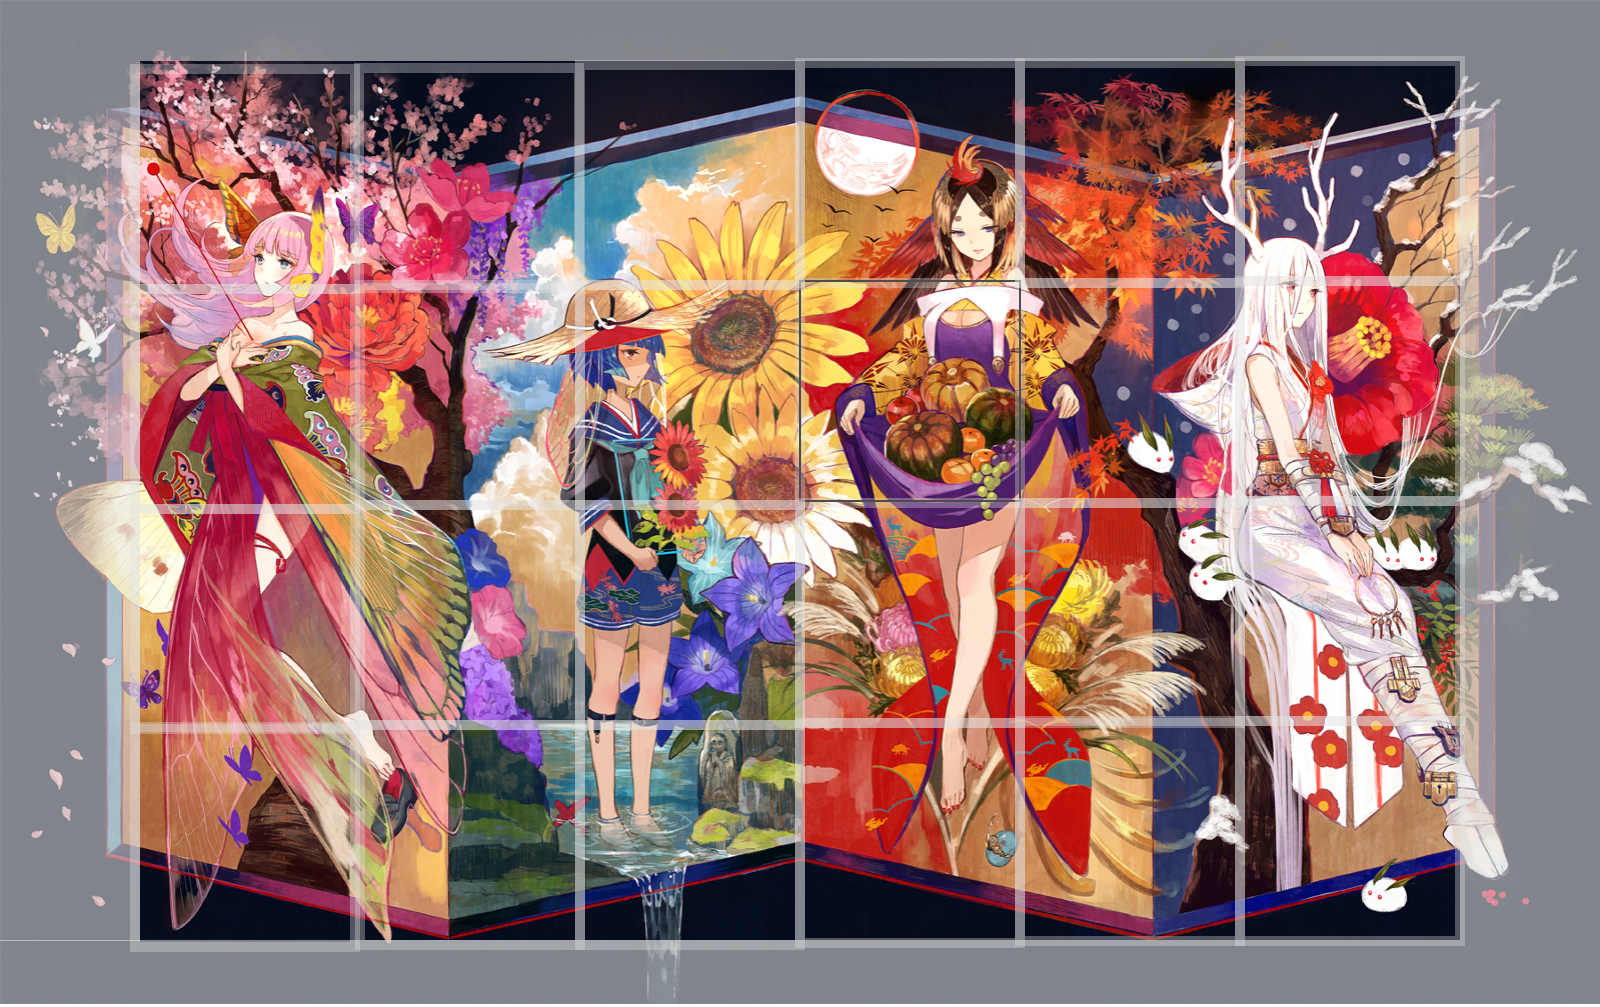
\includegraphics[width=0.5\linewidth]{crop_sample.png}
  \caption{Samples of cropping the image.}
  \label{crop_sample}
\end{figure}




\section{Conv2D networks}

Hyper parameters include number of layers, filter size, stride and padding number, learning rate and so forth. The input tensor is fed into the model and after each layer (or sublayer) the size of output tensor could be calculated by the following equation:
$$n = \frac{m+2p-f}{s} + 1$$
where m is the size of input tensor, n is the size of output tensor, p is the number of padding number, s is the number of strides.

In the first attempt the Conv2D network only contains 2 layers. Each layer contains 3 sublayers, which are convolutional layer, rectified linear unit layer (ReLU) and max-pooling layer. Also the input training set contains 360 images as is mentioned above, with each image of size 500 x 500 x 3. The input images were first transformed into matrix representation, and then stored in a Numpy array as a whole. This works well with input tensors in TensorFlow.

The first layer contains a convolutional layer of filter size equals 4 x 4 x 3, and there are 8 such filters. Other hyper parameters are: stride equals 1 and padding equals 1. Then the result is passed to an activation function, which is ReLU. Thirdly comes the max pooling sublayer, which has filter size of 8 x 8 with number of stride equals 8 and padding equals 1. After the first layer, each output tensor is of size 16 x 16 x 8.

The second layer contains the filter size equals 2 x 2 x 8. There are 16 filters each is applied to the tensor with 1 stride and 1 padding. The filter in the max pooling sublayer is of size 4 x 4, with stride equals 4 and padding equals 1. After this layer, each output tensor is of size 16 x 16 x 16.

Then each output tensor is flattened and combined in a vector. This vector is the input vector of a fully connected (FC) layer. Corresponding weights are assigned to each entry automatically in TensorFlow. The output of this FC layer is the output of the whole Con2D net.

%/tuuuuuuuuuuuuuuuuuuuuuuuuuuuuuuuuuuuuuuu


\begin{figure}[ht]
  \centering
  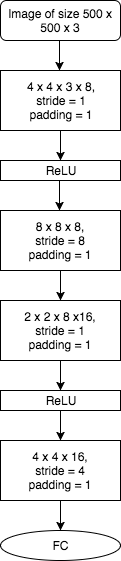
\includegraphics[width=0.2\linewidth]{cnn_structrue_1.png}
  \caption{CNN structrue.}
  \label{cnn_structrue_1}
\end{figure}

\begin{figure}[ht]
  \centering
  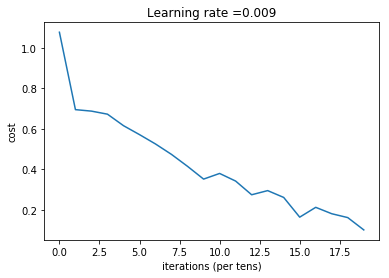
\includegraphics[width=0.6\linewidth]{cnn_structrue_1_result.png}
  \caption{Result 1}
  \label{words segmentation1}
\end{figure}

\begin{figure}[ht]
  \centering
  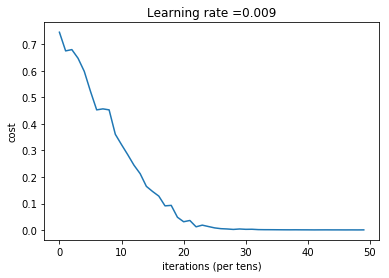
\includegraphics[width=0.6\linewidth]{cnn_structrue_2_result.png}
  \caption{Result 2}
  \label{words segmentation1}
\end{figure}

Set the learning rate to 0.009. After running for 20 epochs, the cost converges. Training accuracy is very high because the network remembers features of every image. But the testing accuracy is only 0.556. This is very bad. It means that when encounter a new image, the network performs just a little bit better than simply ‘guess’ whose author this picture is. Also, the learning process is really slow. For Macbook Air with 1.6 GHz Intel Core i5 and 8 GB RAM, each epoch takes nearly 2 minutes. 

The reason for testing accuracy being small is that the network overfits the training set. And since the whole process took a long time, so we decided to make the input images smaller and then tune the hyper parameters so that the model could fit the images better. Below is the Conv2D net flow chart for our second attempt and its cost.

%/tuuuuuuuuuuuuuuuuuuuuuuuuuuuuuuuuuuuuuuu

The cost converges after 30 epochs and the training process is much faster. Gladly we obtained the training accuracy of up to 0.63. From this we can tell that Conv2D network can more or less  extract unique features of each author, though the feature seems to be vague and implicit.

Then we tried to make the network deeper. We added a new layer to the second layer in the third attempt, but the testing accuracy result is 0.58. To our surprise, adding layer to make the network deeper did not benefit the result. Later we reached accuracy of up to 0.71 for these two authors identification, and Con2D net met its bottleneck.



\section{ResNet}
\subsection{Implement}

Deeper neural networks are more difficult to train. A residual learning framework (ResNet) could ease the training of networks that are substantially deeper than those used previously. ResNet explicitly reformulate the layers as learning residual functions with reference to the layer inputs, instead of learning unreferenced functions. ResNets use residual blocks to ensure that upstream gradients are propagated to lower network layers, aiding in optimization convergence in deep networks [7].


Our second network is the ResNet-14 network with fullyconnected layer. The model is trained from scratch to learn features solely from our dataset.     The network architecture is shown in Figure \ref{resnet}. We used the 14-layer version of ResNet for faster training and decreasing the memory usage due to the limit of our computer.

\begin{figure}[ht]
  \centering
  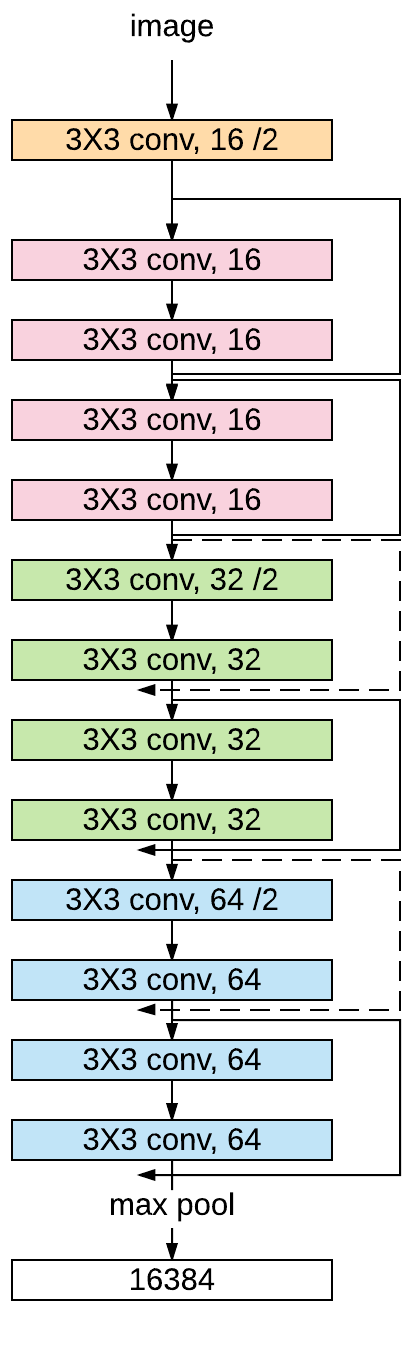
\includegraphics[width=0.3\linewidth]{resnet.png}
  \caption{ResNet-14.}
  \label{resnet}
\end{figure}

\subsection{Experiment}
We first use $250 \times 250 \times 3$ size image from 9 different artists (each artist contributes 800 images) to train the model. The result is shown in \ref{resnet_accuracy}. With the increaing of training steps, the training accuracy increases until 1. But the test accuracy is around 28\% finally. The perfermance is bad, but better than randomly assgin a class (arrcuracy = $\frac{1}{9}$).The overfit might due to the lack of images or the complexicity of the model.

\begin{figure}[ht]
  \centering
  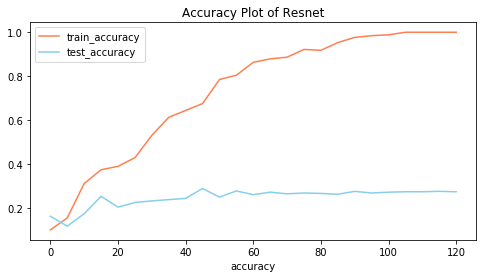
\includegraphics[width=0.6\linewidth]{resnet_accuracy.png}
  \caption{ResNet Accuracy}
  \label{resnet_accuracy}
\end{figure}

Then we try $100 \times 100 \times 3$ size image from 9 different artists (each artist contributes 4000 images) and delete 4 layers before max pool. But the result is not better. It might because we didn't remove the images that only contains same color and no other information. Since most of the image is drawn directly in the computer, there are many pure color cropped images.

We try to let the ResNet to only determine two artists and something interesting happens. We combined the first nine authors in pairs and train the model using $250 \times 250 \times 3$ size images from the two artists (each artist contributes 800 images). The test accuracy varies from 0.559 - 0.957 as shown in Table \ref{my-label}. It seems that some artists have strong personal style and some artists have similar styles. Artist 2 has accuracy rate above 80\% with all other artist. We check the images by human eye and see that artist 2 has strong personal style and his/her iamges are easily to be distingush from other artists' images. We also check he images of artist 6 and 7 which has highest accuracy 0.957627. The main difference between the two artist is that 6 uses light color and 7 uses dark color.



\begin{table}[]\footnotesize
\centering
\caption{My caption}
\label{my-label}
\begin{tabular}{@{}llllllllll@{}}
\toprule
  & 0        & 1        & 2        & 3        & 4        & 5        & 6        & 7        & 8 \\ \midrule
0 & -        &          &          &          &          &          &          &          &   \\
1 & 0.559322 & -        &          &          &          &          &          &          &   \\
2 & 0.872881 & 0.90678  & -        &          &          &          &          &          &   \\
3 & 0.720339 & 0.786667 & 0.805085 & -        &          &          &          &          &   \\
4 & 0.559322 & 0.659864 & 0.876712 & 0.720339 & -        &          &          &          &   \\
5 & 0.838983 & 0.78169  & 0.851064 & 0.671429 & 0.669492 & -        &          &          &   \\
6 & 0.847458 & 0.897436 & 0.825806 & 0.707792 & 0.711409 & 0.635593 & -        &          &   \\
7 & 0.694915 & 0.844156 & 0.875817 & 0.815789 & 0.80916  & 0.896825 & 0.957627 & -        &   \\
8 & 0.895161 & 0.860294 & 0.903704 & 0.873134 & 0.888889 & 0.871253 & 0.885714 & 0.813559 & - \\ \bottomrule
\end{tabular}
\end{table}


\section{Conclusion and Future Work}

\subsection{Conclusion}
Based on our implementation and the attempt of hyper-parameters and different network, for Convolution Neural Network, the accuracy for two classes' identification is 0.56. But for Resnet, for the same classes' identification is also 0.559 which is only a little bit higher than the normal CNN network. But we test for the different classes' and found that the range of the accuracy for different classes' identification differs a lot, range from 0.559 - 0.957. The above results means that the accuracy depends very much on the chosen of authors. There are several reasons that the performance of the system is not good at all, one of the reason is that the dataset is quite small, for every authors we only have 200 pictures, this limited size of the dataset makes the work harder. So we divide every picture into four parts, trying to increase the number of the dataset, this helps a little to the system, the accuracy for two classes' identification raises from 0.56 to 0.625. Another reason is most figures under Japanese artist looks the very similar, big eye and small faces lolita with no obvious character's distinct features, let alone with that the images losses the brashes and strokes' characteristic due to that some authors prefer draw electronically. So Frankly speaking, the Anime Artist Analysis is a hard topic. 
    
\subsection{Future Work}
Based on the low accuracy of the results from both traditional Convolution Neural Network and Residential Network, there are several ways that we think up to improve the performance of our identification and classification system. 

So first, the most straightforward way is to test other hyper-parameters. And then we'd like to try to train the system by VGG network. VGG net always set the filter size as $3*3$, and used $2*2$ pooling size, and doubling the the number of filters after each pooling through out the whole network. VGG is a network that indicates that the deeper the better, so it will be slow to train the data. Actually this is already an on-going process, we started training our images by VGG net but it seems like VGG network has a high requirement on the hardware, so based on our laptop it seems really difficult to train to images and finished the process. 

Another things that we could do is to increase our dataset size, crawling more images so that letting the system learn more.

\subsubsection*{Acknowledgments}
This research was creative due to Machine Learning course taught by Manfred K. Warmuth, Professor in Computer Science Department at University of California, Santa Cruz. I want to thank the professor for giving us an opportunity to implement the project, as well as imparting so many interesting knowledge. And I also want to thanks the teaching assistant of the course, Ehsan Amid and Tianyi Luo, who give us a lot of useful advices.






\section*{References}

  
[1] Alexander, J.A.\ \& Mozer, M.C.\ (1995) Template-based algorithms
for connectionist rule extraction. In G.\ Tesauro, D.S.\ Touretzky and
T.K.\ Leen (eds.), {\it Advances in Neural Information Processing
  Systems 7}, pp.\ 609--616. Cambridge, MA: MIT Press.

[2] Bower, J.M.\ \& Beeman, D.\ (1995) {\it The Book of GENESIS:
  Exploring Realistic Neural Models with the GEneral NEural SImulation
  System.}  New York: TELOS/Springer--Verlag.

[3] Hasselmo, M.E., Schnell, E.\ \& Barkai, E.\ (1995) Dynamics of
learning and recall at excitatory recurrent synapses and cholinergic
modulation in rat hippocampal region CA3. {\it Journal of
  Neuroscience} {\bf 15}(7):5249-5262.
  
[4]Z. A. M. X. Bosch, A. Image classification using rois and multiple kernel learning, 2008. [16]S. Lazebnik, C. Schmid, and J. Ponce. Beyond bags of features: Spatial pyramid matching for recognizing natural scene categories, 2006.

[5] K. He, X. Zhang, S. Ren, and J. Sun. Deep residual learning for image recognition. arXiv preprint, abs/1512.03385,
2015.
 
[6]T. E. Lombardi. The classification of style in fine-art painting. ETD Collection for Pace University, 2005. 

[7]D. G. Lowe. Distinctive image features from scale-invariant keypoints., 2004. 

[8] J. Jou and S. Agrawal. Artist identification for renaissance paintings.

\end{document}
